\chapter{Kelengkapan Internship dan Tugas Akhir}

\section{Tahapan Pergantian Judul}
Lhat pada gambar \ref{figure:P2}.
\begin{figure}[ht]
	\centerline{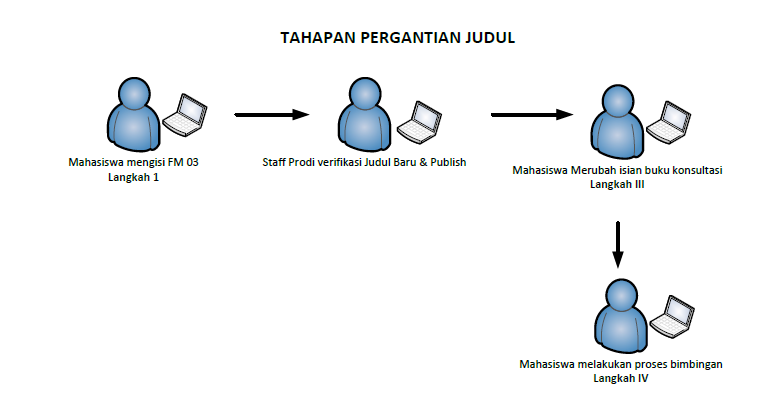
\includegraphics[width=1\textwidth]{figures/ganti_judul.png}}
	\caption{Tahapan Pergantian Judul}
	\label{figure:P2}
	\end{figure}

\section{Tahapan Pengajuan Sidang}
Lhat pada gambar \ref{figure:P3}.
\begin{figure}[ht]
	\centerline{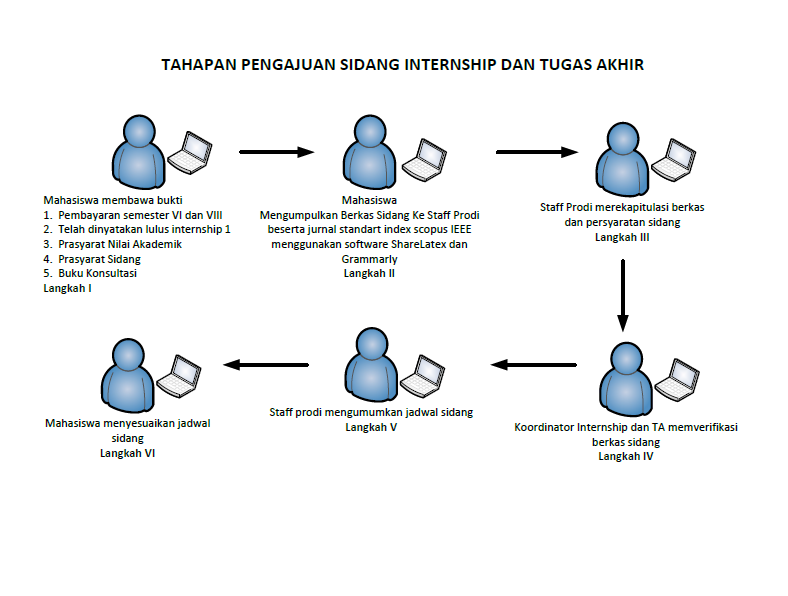
\includegraphics[width=1\textwidth]{figures/draft.png}}
	\caption{Tahapan Pengajuan Sidang}
	\label{figure:P3}
	\end{figure}
\section{Tahapan Revisi Laporan dan Jurnal}
Lhat pada gambar \ref{figure:P31}.
\begin{figure}[ht]
	\centerline{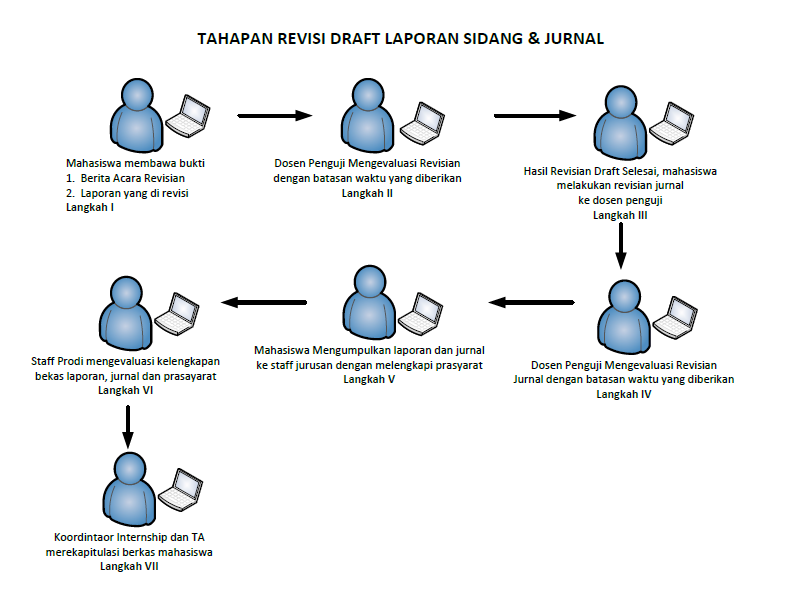
\includegraphics[width=1\textwidth]{figures/revisi.png}}
	\caption{Tahapan Revisi Laporan dan Jurnal}
	\label{figure:P31}
	\end{figure}
\section{Tahapan Sidang Ulang}
Lhat pada gambar \ref{figure:P4}.
\begin{figure}[ht]
	\centerline{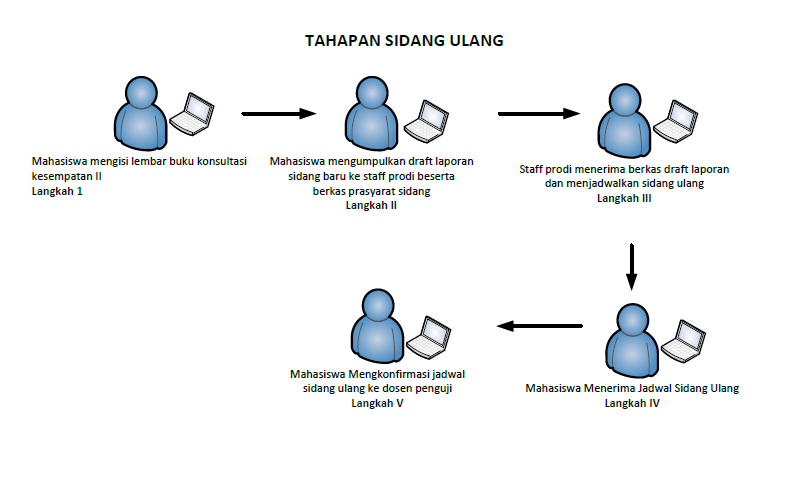
\includegraphics[width=1\textwidth]{figures/ulang.png}}
	\caption{Tahapan Sidang Ulang}
	\label{figure:P4}
	\end{figure}
\section{Tahapan Sidang Kode Etik}
Lhat pada gambar \ref{figure:P5}.
\begin{figure}[ht]
	\centerline{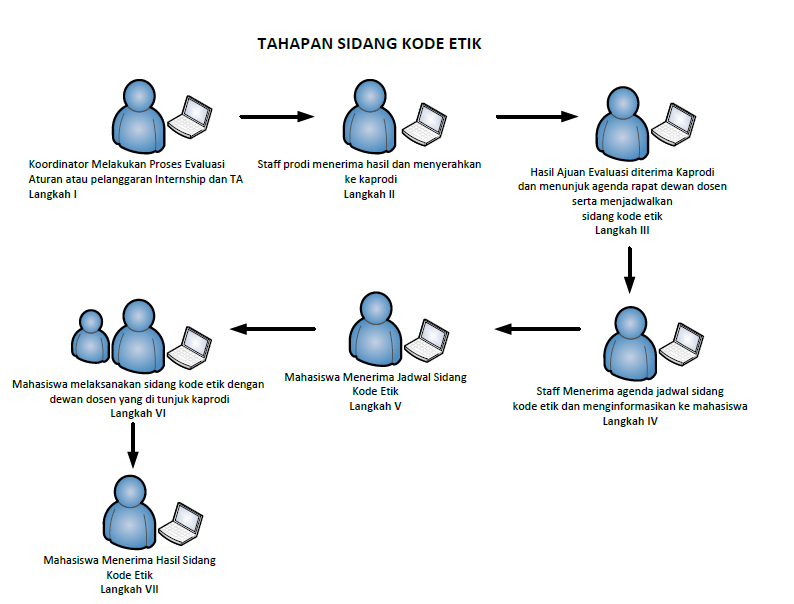
\includegraphics[width=1\textwidth]{figures/kode.png}}
	\caption{Tahapan Sidang Kode Etik}
	\label{figure:P5}
	\end{figure}
	
\chapter{Penutup}

Setiap mahasiswa  diwajibkan mengikuti ketentuan yang ditetapkan dalam buku pedoman ini. Dengan demikian diharapkan akan tercipta keseragaman format dan mutu laporan internship dan tugas akhir di lingkungan Program Studi D4 Teknik Informatika. Sejalan dengan perkembangan ilmu pengetahuan, Pedoman ini akan senantiasa disempurnakan. Oleh sebab itu, saran perbaikan akan dengan senang hati ditampung demi penyempurnaan buku pedoman ini. Hal yang belum diatur dalam pedoman ini akan ditetapkan kemudian.